\documentclass[border=5pt]{standalone}
\usepackage[utf8]{inputenc}
\usepackage{amsmath}
\usepackage{amssymb}

\usepackage{tikz}
\usetikzlibrary{shapes.geometric, arrows}

\tikzstyle{startstop} = [rectangle, rounded corners, minimum width=3cm, minimum height=1cm,text centered, draw=black, fill=red!30]
\tikzstyle{io} = [trapezium, trapezium left angle=70, trapezium right angle=110, minimum width=3cm, minimum height=1cm, text centered, draw=black, fill=blue!30]
\tikzstyle{process} = [rectangle, minimum width=3cm, minimum height=1cm, text centered, draw=black, fill=orange!30]
\tikzstyle{decision} = [diamond, minimum width=3cm, minimum height=1cm, text centered, draw=black, fill=green!30]
\tikzstyle{arrow} = [thick,->,>=stealth, rounded corners]
\tikzstyle{fdot} = [circle, minimum width=4pt, fill]
\tikzstyle{line} = [thick,>=stealth, rounded corners]

\begin{document}

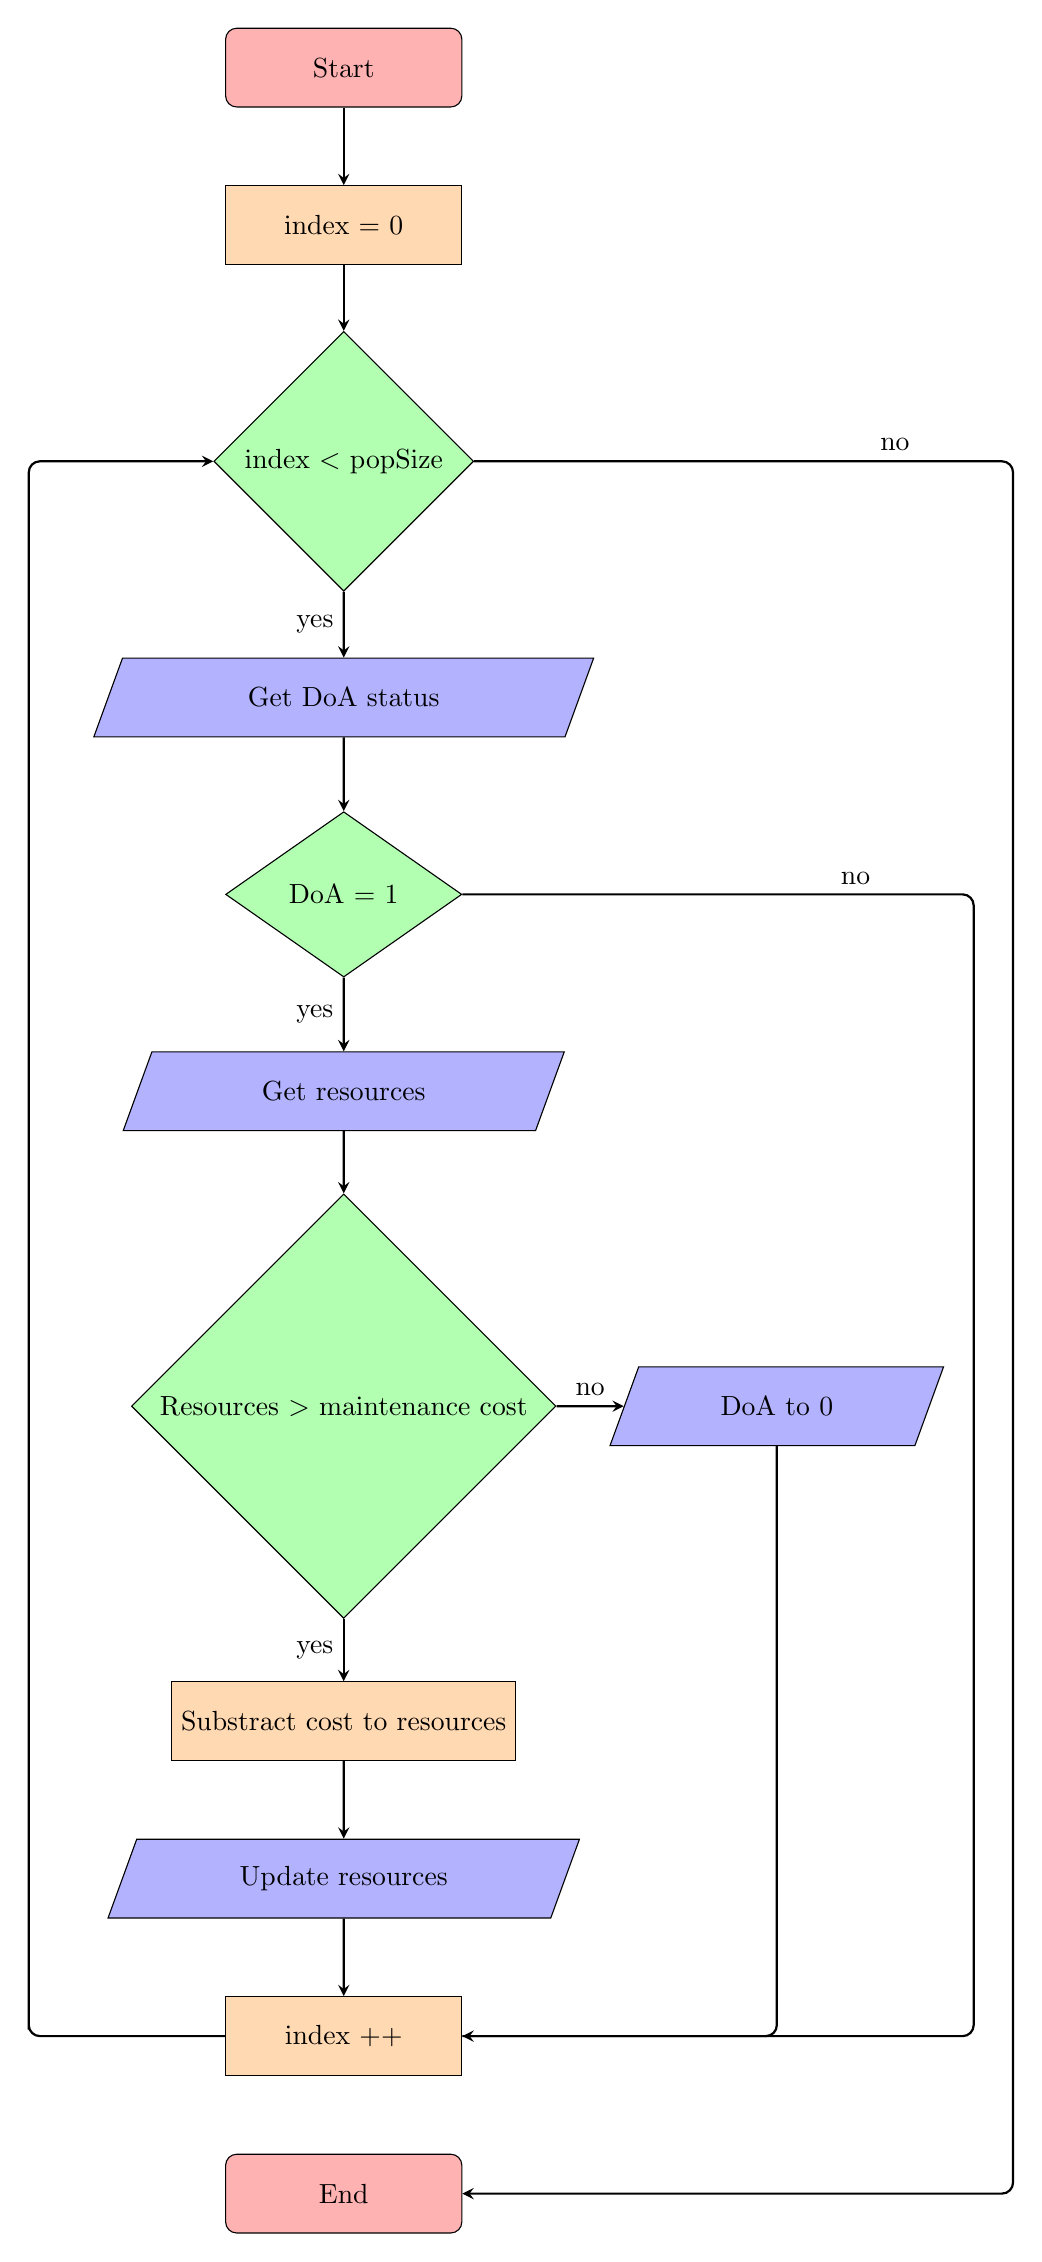
\begin{tikzpicture}[node distance=3cm]

\node (start) [startstop] {Start};
\node (pro1) [process, below of=start, yshift=1cm] {index = 0};
\node (dec1) [decision, below of=pro1] {index $<$ popSize};
\node (in1) [io, below of=dec1] {Get DoA status};
\node (dec2) [decision, below of=in1, yshift=0.5cm] {DoA $=$ 1};
\node (in2) [io, below of=dec2, yshift=0.5cm] {Get resources};
\node (dec3) [decision, below of=in2, yshift=-1cm] {Resources $>$ maintenance cost};
\node (out1) [io, right of=dec3, xshift=2.5cm] {DoA to 0};
\node (pro2) [process, below of=dec3, yshift=-1cm] {Substract cost to resources};
\node (out2) [io, below of=pro2, yshift=1cm] {Update resources};
\node (pro3) [process, below of=out2, yshift=1cm] {index ++};
%\node (fdot1) [fdot, right of=pro3, xshift=2.5cm] {};
\node (stop) [startstop, below of=pro3, yshift=1cm] {End};

\draw [arrow] (start) -- (pro1);
\draw [arrow] (pro1) -- (dec1);
\draw [arrow] (dec1) -- node[anchor=east] {yes} (in1);
\draw [arrow] (dec1) -| node[anchor=south, xshift=-1.5cm] {no} + (8.5,-0.5) |- (stop);
\draw [arrow] (in1) -- (dec2);
\draw [arrow] (dec2) -- node[anchor=east] {yes} (in2);
\draw [line] (dec2) -| node[anchor=south, xshift=-1.5cm] {no} + (8,-0.5) |- (pro3);
\draw [arrow] (pro3) -| + (-4,0) |- (dec1);
\draw [arrow] (out1) |- (pro3);
%\draw [arrow] (fdot1) -- (pro3);
\draw [arrow] (in2) -- (dec3);
\draw [arrow] (dec3) -- node[anchor=east] {yes} (pro2);
\draw [arrow] (dec3) -- node[anchor=south] {no} (out1);
\draw [arrow] (pro2) -- (out2);
\draw [arrow] (out2) -- (pro3);

\end{tikzpicture}

\end{document}